%\nonstopmode

\documentclass[11pt]{article}

\usepackage{mathenv}
\usepackage{cancel}
\usepackage{fullpage}
\usepackage{amsmath}
\usepackage{amsfonts}
\usepackage{ulem}
\usepackage{graphicx}
\usepackage{verbatim}
\usepackage{apalike}
\usepackage{algorithm}
\usepackage{algorithmic}
\usepackage[usenames, dvipsnames]{color}
\usepackage[colorlinks=true, linkcolor=OliveGreen, citecolor=Purple]{hyperref}

\newcommand{\paperlink}[1]{\href{/Users/adkein/Documents/papers/#1.pdf}{\cite{#1}}}
\newcommand{\booklink}[2]{\href{/Users/adkein/Documents/books/#2.pdf}{\cite{#2}}}
\newcommand{\doh}{\partial}
\newcommand{\constant}{\text{ const. }}
\newcommand{\mc}{\mathcal}
\newcommand{\mb}{\mathbb}
\newcommand{\ds}{\displaystyle}
\newcommand{\ts}{\textstyle}

\allowdisplaybreaks

\begin{document}

\title{Lab notebook: DDPM object tracking}
\author{Carl Smith}
\date{April 11, 2012 - June 4, 2012}
\maketitle
%\tableofcontents

\section*{Notes}
\addcontentsline{toc}{section}{Notes}

\subsection*{Thursday, May 31, 2012}
In fact, the transition kernel doesn't have to use the same $\{\mu_i\}$'s at all. We can have
%
\begin{align*}
p(\theta_t|\theta_{t-1}) \propto \sum_i e^{\kappa \mu_i^T\mathbf{h}_{t-1}} e^{\kappa \nu_i^T \mathbf{h}_t}
\end{align*}

\subsection*{Tuesday, May 29, 2012}

A thought: you can construct transition kernels that encourage cyclic motion, like the following:
%
\begin{align*}
p(\theta_t|\theta_{t-1}) \propto \sum_i e^{\kappa \mu_i^T \mathbf{h}_{t-1}} e^{\kappa \mu_{i+1}^T \mathbf{h}_t}
\end{align*}
%
where the $\{\mu_i\}$ are organized in, e.g., a circular path around the sphere.

Okay, so I think I have found a way to construct stationary distributions whose modes have different concentration parameters. The trick is that we also have to change the weights of the modes just so. Say that our stationary distribution is
%
\begin{align*}
\mathbb{G}_0(\theta) \propto \sum_i \alpha_i e^{\kappa_i \mu^T \mathbf{h}}
\end{align*}
%
where to be concrete we constrain the $\{\alpha_i\}$ to sum to one. And suppose we have the same transition kernel from Equation \eqref{eq:transition_kernel}. Then, following Equation \eqref{eq:stationary_distribution}, we require for stationarity that
%
\begin{align*}
\sum_j \alpha_j \frac{||\kappa_i\mu_i + \kappa_j\mu_j||}{4\pi\sinh(||\kappa_i\mu_i+\kappa_j\mu_j||)} = \alpha_i \;\;\; \forall i
\end{align*}
%
In fact, in this case we're free to choose the directions $\{\mu_i\}$ however we please, so long as we use the same $\{\mu_i\}$ for the transition kernel and so long as we vary the $\{\kappa_i\}$ and $\{\alpha_i\}$ appropriately. (Another question is, can we also allow for using different $\{\kappa_i\}$ for the stationary distribution and for the transition kernel?)

\subsection*{Wednesday, May 9, 2012}

First off, Equation \eqref{eq:stationary_distribution} may be correct after all, so long as the sum over $j$ is the same for each $i$. Such is the case, as already mentioned, if the modes lie on the vertices of a Platonic solid inscribed in the sphere.

Met with Frank today. He wants to figure out a way to vary the $\kappa$'s in the von Mises-von Mises transition kernel and/or stationary distribution. Also he'd like to see samples from the generative model. First I'll have to figure out how to sample from a multivariate von Mises distribution.

I've found \texttt{randvonMisesFisherm.m} by Sungkyu Jung, which samples from the von Mises-Fisher distribution of arbitrary dimension.

For our stationary distribution, we're constrained to keep the modes on the sphere symmetric. That is, rotating the sphere in any way that leaves the positions of the (indistinguishable) modes the same must be an identity element. For instance, we can inscribe any Platonic solid in the sphere and put modes at its vertices. Then we get a distribution that looks like Figure \ref{fig:vm-draws__n_1e5__k_1} for 10,000 samples with $\kappa=1$, and like Figure \ref{fig:vm-draws__n_1e5__k_10} for 10,000 samples with $\kappa=10$, where in the latter the segregation into modes is obvious, but the former distribution looks pretty uniform to me. These are for the modes being placed on the vertices of an inscribed octahedron, i.e. simply on the axes. Figures \ref{fig:vm-walk__k_1__t_10}, \ref{fig:vm-walk__k_10__t_10}, and \ref{fig:vm-walk__k_100__t_10} show random walks via the octahedral transition kernel with varying $\kappa$ and 10 time steps. As expected, for higher $\kappa$ the walker is effectively trapped in one mode. These were all hand picked so that most of the density was on the side of the sphere facing the viewer.

In other news, it is fine for the stationary distribution to have a different $\kappa$ from that of the transition kernel, i.e.
%
\begin{align*}
\mathbb{G}_0(\theta) \propto \sum_i e^{\kappa_s \mu_i^T \mathbf{h}}
\end{align*}

\noindent where as usual $\mathbf{h}$ is the unit vector in 3-space corresponding to the angle(s) $\theta$, while
%
\begin{align}
\label{eq:transition_kernel}
P(\theta_{t+1} | \theta_{t}) &= \sum_{z_t}^R p(z_t|\theta_t) p(\theta_{t+1}|z_t) \notag \\
&\propto \sum_{z_t}^R e^{\kappa_t \mu_{z_t}^T \mathbf{h_{t+1}}} e^{\kappa_t \mu_{z_t}^T \mathbf{h_{t}}}.
\end{align}

\noindent But, different $\kappa$'s for the different modes? I don't think there's a stationary distribution in that case.

\begin{figure}[h!]
\centering
\includegraphics[scale=0.35]{../fig/vm-draws__n_1e5__k_1.pdf}
\caption{10,000 draws on the octahedral von Mises sphere with $\kappa=1$.}
\label{fig:vm-draws__n_1e5__k_1}
\end{figure}
% Generated using generate_path.m

\begin{figure}[h!]
\centering
\includegraphics[scale=0.35]{../fig/vm-draws__n_1e5__k_10.pdf}
\caption{10,000 draws on the octahedral von Mises sphere with $\kappa=10$.}
\label{fig:vm-draws__n_1e5__k_10}
\end{figure}
% Generated using generate_path.m

\begin{figure}[h!]
\centering
\includegraphics[scale=0.35]{../fig/vm-walk__k_1__t_10.pdf}
\caption{10 steps of random walk on octahedral von Mises sphere with $\kappa=1$.}
\label{fig:vm-walk__k_1__t_10}
\end{figure}
% Generated using generate_path.m

\begin{figure}[h!]
\centering
\includegraphics[scale=0.35]{../fig/vm-walk__k_10__t_10.pdf}
\caption{10 steps of random walk on octahedral von Mises sphere with $\kappa=10$.}
\label{fig:vm-walk__k_10__t_10}
\end{figure}
% Generated using generate_path.m

\begin{figure}[h!]
\centering
\includegraphics[scale=0.35]{../fig/vm-walk__k_100__t_10.pdf}
\caption{10 steps of random walk on octahedral von Mises sphere with $\kappa=100$.}
\label{fig:vm-walk__k_100__t_10}
\end{figure}
% Generated using generate_path.m

\subsection*{Monday, April 30, 2012}
It seems to be important, in coming up with a stationary distribution $\mb{G}_0$ to have a uniform grid of points on the (hyper-)sphere. One thing I've come across in the 3D case is inscribing an icosahedron and taking the vertices to be the grid points. Unfortunately this rather fixes the resolution of the smoothing, so that's not the most desirable. It would be preferable to somehow write down a stationary distribution for the normal latitude-longitude grid.

Maybe, and I'm not sure why I ruled this out before, the stationary density is simply uniform on the sphere:

\begin{align*}
\int d\theta_{t-1} \mb{G}_0(\theta_{t-1}) &\sum_i p(\mu_i|\theta_{t-1})p(\theta_t|\mu_i) \\
&\propto \int d\theta_{t-1} \sum_i e^{\kappa \mu_i^T\mathbf{h}_t} e^{\kappa\mu_i^T\mathbf{h}_{t-1}} \\
\end{align*}

\noindent Nope.

\subsection*{Thursday, April 26, 2012}
On the unit circle, the von Mises distribution can be parametrized by the ``mean" angle $\phi$ where the mode of the density resides:
%
\begin{align*}
f(x|\phi,\kappa) &= \frac{e^{\kappa\cos(x-\phi)}}{2\pi I_0(\kappa)}
\end{align*}

\noindent where $I_0(x)$ is the order 0 modified Bessel function. (Assume throughout that $\kappa$ is fixed.) Instead, however, consider the unit vector $\mathbf{x}$ from the circle's center to the point on the perimeter an angle $x$ away from the $x$-axis. Similarly define $\mathbf{\mu}$ to be the vector with tail at the circle's center and point on the perimeter making the angle $\phi$ with the $x$-axis. This we may write
%
\begin{align*}
f(\mathbf{x}|\mathbf{\mu},\kappa) = \frac{e^{\kappa \mathbf{\mu}^T \mathbf{x}}}{2\pi I_0(\kappa)}.
\end{align*}

In the same vein, for higher dimensional $\mathbf{x}$ we have the von Mises-Fisher distribution:
%
\begin{align*}
f_p(\mathbf{x};\mu,\kappa) &= C_p(\kappa) e^{\kappa \mu^T \mathbf{x}}
\end{align*}

\noindent where $C_p(\kappa)$ is a normalization constant that involves Bessel functions of $\kappa$. ($p=2$ for the simple von Mises distribution on the circle.)

In \paperlink{Neiswanger_2012} we have that we need to choose $\mb{G}_0(\theta)$, $p(\theta|z)$, and $p(z|\theta)$ such that 
%
\begin{align*}
\int &\mb{G}_0(\theta_{t-1}) P(\theta_t|\theta_{t-1})d\theta_{t-1} \\
 &= \int \mb{G}_0(\theta_{t-1}) \sum_z P(\theta_t|z_t)P(z_t|\theta_{t-1})d\theta_{t-1} \\
&= \mb{G}_0(\theta_t)
\end{align*}

\noindent To this end, choose the following transition kernel: (Note that $\theta$ denotes some cluster parameter(s) -- the {\it angle} in the distribution. Denote by $\textbf{h}$ the corresponding unit vector in the $p$-dimensional space.)
%
\begin{align*}
p(\theta_t|\theta_{t-1}) \propto \sum_i e^{\kappa \mu_i^T \mathbf{h_t}} e^{\kappa \mu_i^T \mathbf{h_{t-1}}}
\end{align*}

\noindent where the $\{\mu_i\}$ form a grid in angle-space. (Imagine a point on a globe wherever a latitude and longitude line intersect. This obviously results in anisotropic coverage of the sphere. We'll return to this point below.)

Then the inner products to be computed are of the form
%
\begin{align*}
\int d\theta \; e^{\kappa(\mu_i+\mu_j)^T\mathbf{h}} =C_p\left(\kappa\cdot||\mu_i+\mu_j||\right)
\end{align*}

The stationary distribution $\mb{G}_0$ puts equal density on each bump:
%
\begin{align*}
\xcancel{\mb{G}_0(\theta_t) = \sum_i e^{\kappa \mu_i^T \mathbf{h}_t}}
\end{align*}
%
\begin{align}
\int d\theta_{t-1} &\mb{G}_0(\theta_{t-1}) \sum_i p(\mu_i|\theta_{t-1})p(\theta_t|\mu_i) \notag \\
&\propto \int d\theta_{t-1} \sum_{ij} e^{\kappa \mu_i^T \mathbf{h}_t} e^{\kappa \mu_j^T\mathbf{h}_{t-1}} e^{\kappa \mu_i^T\mathbf{h}_{t-1}} \notag \\
&\propto \sum_{ij} C_p\left(\kappa\cdot||\mu_i+\mu_j||\right) e^{\kappa \mu_i^T \mathbf{h}_t} \notag \\
&\xcancel{\propto \sum_{i} e^{\kappa \mu_i^T \mathbf{h}_t} = \mb{G}_0(\theta_t)}
\label{eq:stationary_distribution}
\end{align}

\noindent That last step follows because for each $i$, the range of values taken by $||\mu_i+\mu_j||$ is the same, and so the entire $\sum_j C_p$ coefficient is a common factor.

\subsection*{Wednesday, April 11, 2012}
Frank thinks the low-rank models ideas can straightforwardly be applied to his work with an undergraduate described in \paperlink{Neiswanger_2012}. I met with him March 8 and here are some notes from that meeting and an email I sent him:

These cluster parameters $\theta_{k,t}$ change over time. And the cluster parameters change smoothly; adjacent parameters are coupled using auxiliary variables $z_{k,t,m}$. So we have in mind this graphical model like in Figure \ref{fig:gm1}. Actually these particular distributions aren't important. What is important is that $\theta_{k,t}\approx \theta_{k,t-1}\;\;\forall k$. But there are a couple GPUDDP caveats. We need that $\theta_{k,t}$ can be analytically integrated out given observations: we need to be able to compute $\int d\theta_{k,t} p(x|\theta_{k,t}) G_0(\theta_{k,t}|\theta)$, where $G_0(\theta)$ is the stationary distribution of $p(\theta_{t+1}|\theta_t)$. The question is, can you meet this requirement for arbitrary $F(\theta_{k,t})=p(x_{k,t+1}|\theta_{k,t})$? for $F$ from an exponential family? for $F$ normal?

\begin{figure}[h]
\centering
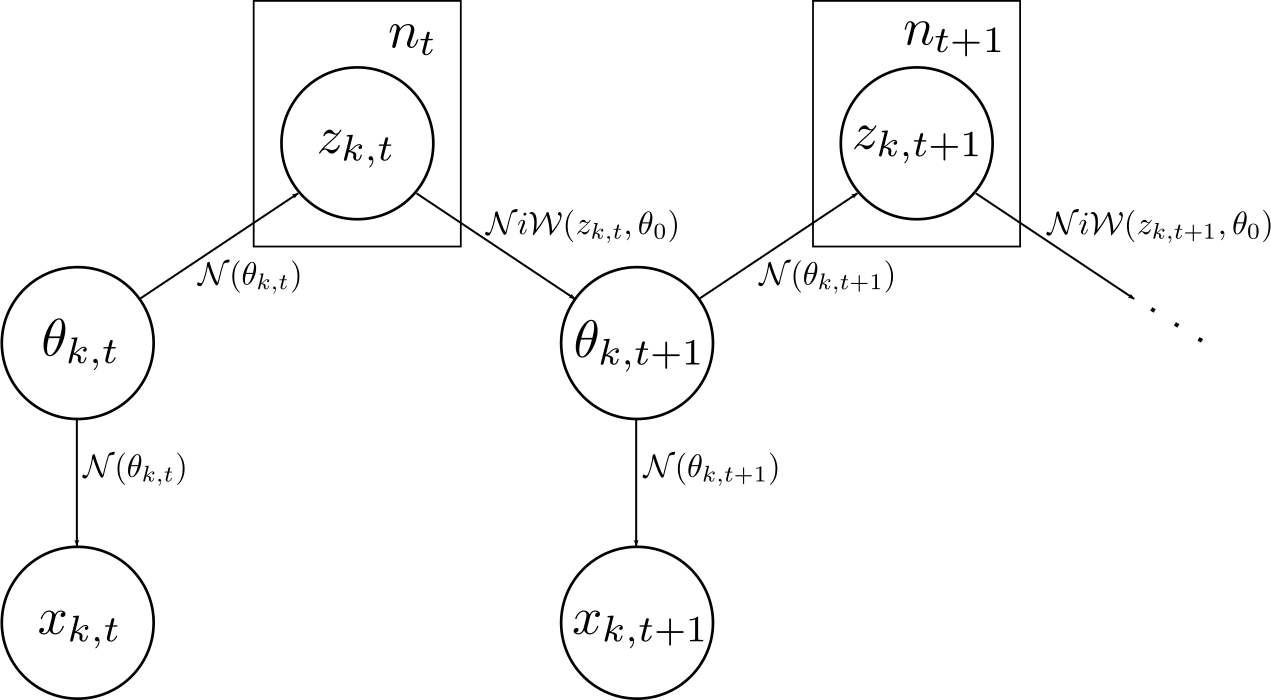
\includegraphics[scale=0.35]{../fig/directed_gm.pdf}
\caption{Cluster parameters $\theta_{k,t}$ vary smoothly over time, enforced by the $z_{k,t,m}$'s.}
\label{fig:gm1}
\end{figure}

What are these parameters exactly? Is $\theta_{k,t}$ the mean and variance of the Gaussian or do we assume unit variance or something? And what are the parameters of the normal inverse Wishart? The normal-inverse-Wishart is parametrized in terms of hyperparamters $(\mu_0, \Lambda_0/\kappa_0; \nu_0, \Lambda)$:

\begin{align*}
\Sigma &\sim \text{Inv-Wishart}_{\nu_0} (\Lambda_0^{-1}) \\
\mu|\Sigma &\sim \mathcal{N}(\mu_0,\Sigma/\kappa_0)
\end{align*}

\noindent So how do the $z$'s and $\theta$'s relate to these? {\it Update: see \paperlink{Neiswanger_2012} for all these details.}


\bibliographystyle{apalike}
\bibliography{refs}
\end{document}
